\documentclass[tikz,border=6pt]{standalone}
\usepackage{amsmath}
\usetikzlibrary{positioning}
\makeatletter
\AtBeginDocument{\global\let\pgf@selectfontorig\relax}
\makeatother

\begin{document}
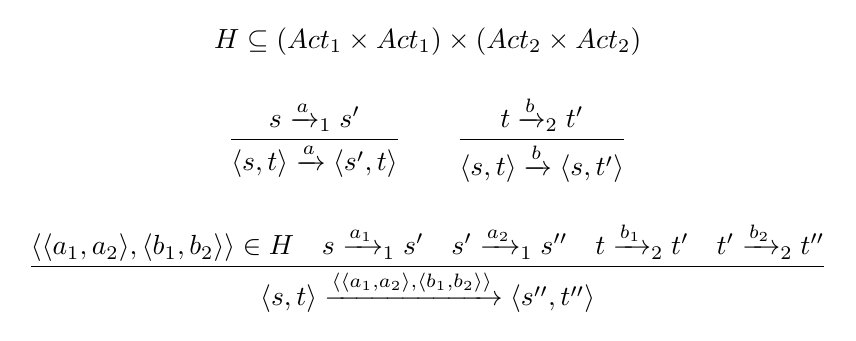
\begin{tikzpicture}
\node[inner sep=0pt, anchor=west] (hdef) at (0,0)
  {$H\subseteq (Act_1\times Act_1)\times(Act_2\times Act_2)$};
\node[inner sep=0pt, below=5mm of hdef] (base) {
$\displaystyle
\frac{s \xrightarrow{a}_1 s'}{\langle s,t\rangle\xrightarrow{a}\langle s',t\rangle}
\qquad
\frac{t \xrightarrow{b}_2 t'}{\langle s,t\rangle\xrightarrow{b}\langle s,t'\rangle}
$};
\node[inner sep=0pt, below=5mm of base] {
$\displaystyle
\frac{\langle\langle a_1,a_2\rangle,\langle b_1,b_2\rangle\rangle\in H
\quad s\xrightarrow{a_1}_1s'\quad s'\xrightarrow{a_2}_1s''
\quad t\xrightarrow{b_1}_2t'\quad t'\xrightarrow{b_2}_2t''}
{\langle s,t\rangle
\xrightarrow{\langle\langle a_1,a_2\rangle,\langle b_1,b_2\rangle\rangle}
\langle s'',t''\rangle}
$};
\end{tikzpicture}
\end{document}
